%! Author = Matt
%! Date = 3/17/2022

% Preamble
\documentclass[11pt]{article}

\usepackage{hyperref}
\usepackage{csquotes}
\usepackage{pdfpages}
\title{About Bachelor's Thesis}
\author{Matt Yan}
% Document
\begin{document}

    \maketitle

    My undergraduate program, \textit{Specialization in Mathematics}, in the University of Alberta does not require a
    thesis to graduate.
    Instead, students are required to pass a list of classes and satisfy GPA requirements.
    Please refer to the pages below for the specific course and GPA requirements,
    which are a snapshot of \href{https://calendar.ualberta.ca/preview_program.php?catoid=36&poid=42306&returnto=11345}{the calendar website} hosted by University of Alberta, accessed on March 17, 2022.

    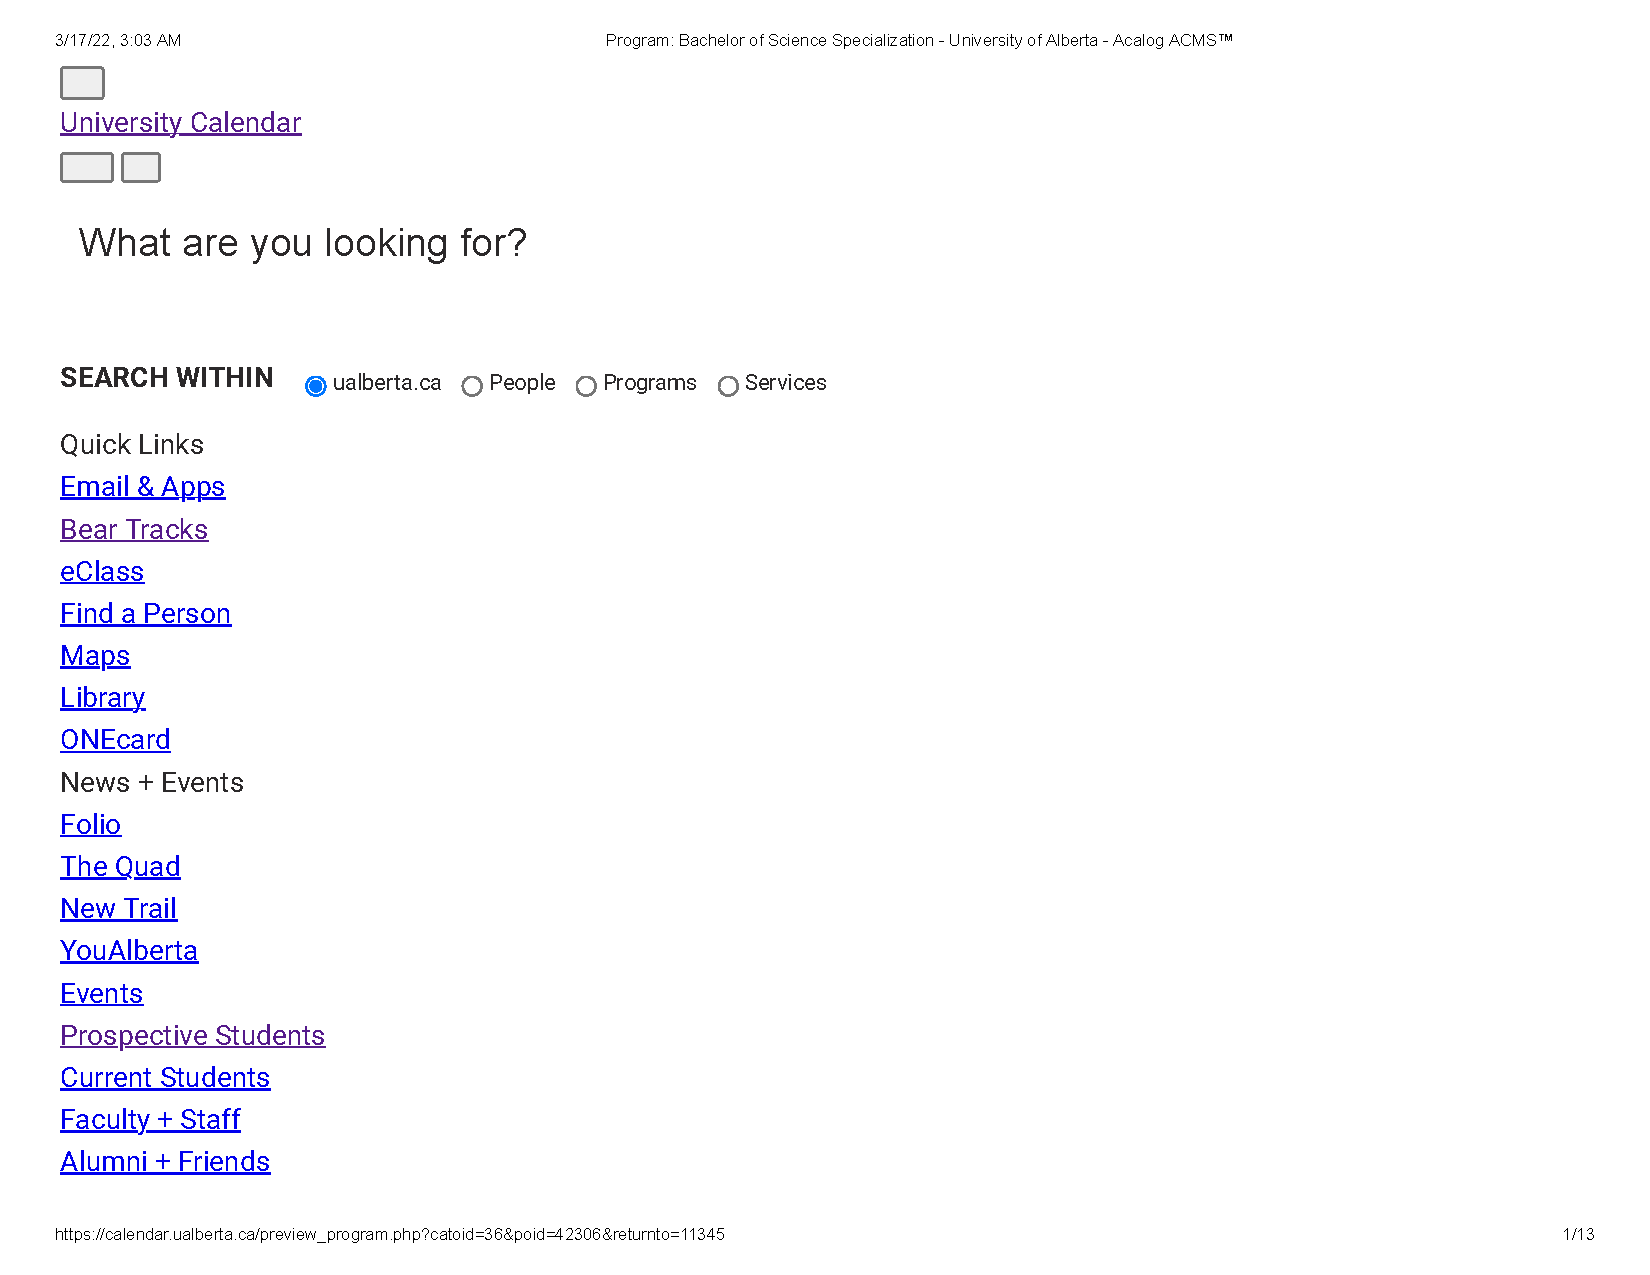
\includepdf[pages=-]{program-bachelor-of-science-specialization-university-of-alberta}

\end{document}